% LaTeX support: latex@mdpi.com
\documentclass[entropy,article,submit,pdftex,oneauthor]{Definitions/mdpi}
\usepackage{booktabs}
\usepackage{needspace}
\firstpage{1}
\makeatletter\setcounter{page}{\@firstpage}\makeatother
\pubvolume{1}\issuenum{1}\articlenumber{0}
\pubyear{2026}\copyrightyear{2026}
\datereceived{ }\daterevised{ }\dateaccepted{ }\datepublished{ }
\hreflink{https://doi.org/}

\Title{Phase-Aware Spectral Entropy as a Diagnostic of Stream-Cipher IV Diffusion: A Shared Effect in Reduced ChaCha20 and Salsa20}
\TitleCitation{Spectral Entropy as an IV-Diffusion Diagnostic}
\Author{Pawe\l{} Augustynowicz $^{1,*}$}
\AuthorNames{Pawe\l{} Augustynowicz}
\AuthorCitation{Augustynowicz, P.}
\address{$^{1}$ \quad Faculty of Cybernetics, Military University of Technology, ul. gen. Sylwestra Kaliskiego 2, 00-908 Warsaw, Poland; pawel.augustynowicz@wat.edu.pl}
\corres{Correspondence: pawel.augustynowicz@wat.edu.pl}

\abstract{Changing an initialization vector should spread its influence through a stream cipher's output. We ask whether spectral entropy of the Hamming weights of output differences from paired IVs can show where that spread is delayed or organized. Across seven ciphers, a graph-matched control and a split into zero-frequency (DC) and varying (AC) power distinguish changes in response size from repeating output patterns. Reduced ChaCha20/2 and Salsa20/2 exhibit a persistent four-position pattern within 512-bit output blocks. In contrast, Grain-128 and Trivium with shortened initialization show IV-response signals that fade in later output blocks. Rotating measurements within each block while preserving their values and DC share removes about 96\% and 94\% of the AC contrast, respectively. An independent scan of all 64 nonce-bit positions confirms a $+0.79059$-bit spectral-entropy gap between Salsa20/2's two nonce words (95\% CI [0.78404, 0.79729]; Holm-adjusted $p=2.0\times10^{-5}$). ChaCha20/2 shows almost no aggregate gap because responses across its 32-bit output words cancel. Standard settings give small contrasts. An auxiliary A5/1 study confirms a zero-clock frame-position gradient but detects no standard-depth response after correction. Notably, simpler statistics also reveal the large deficits in the reduced cores. Spectral decomposition helps explain those signals by separating response size from recurring within-block structure.}
\keyword{spectral entropy; stream ciphers; IV diffusion; Hamming weight; statistical testing; ChaCha20; Salsa20}

\begin{document}
\section{Introduction}

When the initialization vector (IV) changes but the key stays fixed, a stream cipher should spread that change throughout its output. Statistical testing can reveal where that response is delayed, biased, or organized, especially in deliberately reduced configurations. We study the spectral entropy of a concrete response signal: the Hamming weights (HWs) of consecutive output differences between two IVs. This measures how Fourier power is distributed across positions in the observed trajectory. This spectral measure should not be confused with the Shannon entropy of the secret key or the keystream.

The diagnostic is useful only if its components are read correctly. A positive HW trajectory has a large zero-frequency (DC) component, so full-spectrum entropy can respond to the relative size of fluctuations even when the nonzero-frequency (AC) allocation barely changes. Conversely, an AC pattern can be hidden by a larger DC effect. ChaCha20 and Salsa20 generate 512-bit blocks~\citep{nir2018,bernstein2008salsa}. We XOR corresponding blocks from paired nonces and count the changed bits separately in each of four 128-bit segments. This shows whether the response depends on a segment's position within the block. A matched random reference must preserve the reuse of each base IV across masks. Chosen-IV analysis can expose reduced-initialization behavior, but standard and reduced settings answer different questions~\citep{englund2007,fischer2008}.

We ask whether phase-aware spectral entropy can distinguish an IV response that fades after the first output blocks from a pattern that persists, and whether it helps explain each effect. We address this question in four stages. First, we measured Grain-128, Trivium, MICKEY 2.0, HC-128, Rabbit, IETF ChaCha20, and Salsa20 under a common ordinary-IV/nonce measurement protocol~\citep{grain2006,trivium2006,estream2008,nir2018,bernstein2008salsa}. Second, we used matched nonces in ChaCha20 and Salsa20 and rotated HW samples within output blocks to test whether their alignment drives the reduced cores' AC signal. We compared spectral entropy with simpler diagnostics on those same streams. Third, an independent 64-mask experiment measured the effect of every nonce bit and resolved the responses of individual 32-bit output words. Separate fresh-key Grain-128 and Trivium experiments probed effects of shortened initialization. Finally, we tested A5/1, a cipher with published attacks~\citep{biryukov2000}, on the first 114 bits of each frame to see which effects the diagnostic captures. Planned tests were fixed before their respective fresh-key cohorts and evaluated in separate families. We identify exploratory comparisons as descriptive.

\section{Materials and Methods}
\subsection{A Common Ordinary-IV/Nonce Experiment}

For fixed cipher key $K$, configuration $r$, base IV or nonce $v$, and mask $\delta$, let $Z_{K,r}(v)$ and $Z_{K,r}(v\oplus\delta)$ be the first 4096 output bits. Divide each into 32 consecutive, disjoint 128-bit blocks. One trajectory is
\begin{equation}
 h_t=\operatorname{HW}\!\left(Z_{K,r}(v)_{[128(t-1),128t)}\oplus
 Z_{K,r}(v\oplus\delta)_{[128(t-1),128t)}\right),\quad t=1,\ldots,32.
 \label{eq:trajectory}
\end{equation}
Each $h_t$ counts bits changed in one 128-bit output segment. All 32 segments come from the same fixed-key IV pair. For independent uniform 128-bit differences, HW averages 64 without a reproducible pattern over positions. A reduced setting may instead show an early deficit, a recurring position pattern, or both. We compare these responses with a matched control built from the same input pairs.

Each of the seven ciphers was tested with 80 separately derived keys. Separate BLAKE2b domains generate the cipher keys and control secrets~\citep{saarinen2015}, and a dedicated SHAKE256 domain generates four base IVs or nonces per key~\citep{nist2015sha3}. We pair each base input with four single-bit changes, giving 16 IV or nonce pairs per key. We repeat the procedure with four masks that each flip four consecutive bits, forming a second family of 16 pairs. Within a cipher, we use the same pairs at every tested setting, so the inputs stay fixed when settings are compared. Pair count, output length, block width, and estimator are the same across ciphers within each mask family. Key and IV lengths and standard settings vary by cipher (Table~\ref{tab:protocol}).

For an $n$-bit IV or nonce, the single-bit positions are $0$, $\lfloor n/3\rfloor$, $\lfloor2n/3\rfloor$, and $n-1$, with bit 0 the most significant bit of the first byte. Four-bit windows begin at $0$, $\lfloor(n-4)/3\rfloor$, $\lfloor2(n-4)/3\rfloor$, and $n-4$. These positions were fixed before the new keys were generated. They spread changes through each cipher's legal input domain without selecting a mask to maximize a measured effect. We analyze the two mask types separately. Only single-bit masks enter the planned tests.

\begin{table}[H]
\caption{Cipher settings in the common paired-IV/nonce experiment. Key and IV/nonce lengths are in bits. The tested values count the operation shown beside them, and the last value is each cipher's standard setting. For MICKEY 2.0, HC-128, and Rabbit, zero skips only the named final operation. Mandatory key/IV loading or state expansion still occurs.\label{tab:protocol}}
\footnotesize\setlength{\tabcolsep}{4pt}
\begin{tabularx}{\textwidth}{lccXl}
\toprule
\textbf{Cipher} & \textbf{Key/IV (bits)} & \textbf{Tested values} & \textbf{Operation varied} & \textbf{Standard}\\
\midrule
Grain-128 & 128/96 & 0, 32, 64, 128, 192, 256 & Initialization clocks & 256\\
Trivium & 80/80 & 0, 64, 128, 192, 384, 768, 1152 & Initialization clocks & 1152\\
MICKEY 2.0 & 80/80 & 0, 25, 50, 75, 100 & Final blank clocks & 100\\
HC-128 & 128/128 & 0, 256, 512, 768, 1024 & Initialization updates & 1024\\
Rabbit & 128/64 & 0, 1, 2, 3, 4 & IV-setup iterations & 4\\
ChaCha20 & 256/96 & 2, 4, 6, 8, 12, 20 & Core rounds & 20\\
Salsa20 & 256/64 & 2, 4, 6, 8, 12, 20 & Core rounds & 20\\
\bottomrule
\end{tabularx}
\end{table}

All seven standard configurations passed published test vectors or independent library checks. A separate round-by-round implementation also checked the reduced Salsa20 settings.

The tested values do not represent equal amounts of work across ciphers. ChaCha20 and Salsa20 vary core rounds, while the others vary initialization or setup steps. In labels such as Trivium/64 and ChaCha20/2, the number refers to the operation listed in Table~\ref{tab:protocol}. We compare standard configurations under one measurement protocol and interpret each cipher's reduced settings separately.

\subsection{Entropy, Exact Attribution, and Matched Control}

For $Q=16$ trajectories from one key, cipher, configuration, and mask family, we average complete two-sided Fourier powers \emph{before} normalizing:
\begin{equation}
 P_k=\frac1Q\sum_{q=1}^{Q}\left|\operatorname{DFT}(h^{(q)})_k\right|^2,\quad
 p_k=\frac{P_k}{\sum_jP_j},\quad
 H_{\rm MP}=-\sum_{k=0}^{T-1}p_k\log_2p_k,\quad T=32.
 \label{eq:entropy}
\end{equation}
This is entropy in bits of a finite averaged power vector. It measures the spectrum of the IV-response trajectory, not the entropy rate of a keystream or a stationary spectral density. For the tail comparison in Table~\ref{tab:reduced}, we recompute the same statistic from $h_{17},\ldots,h_{32}$ with $T=16$ for both cipher and control. Let $p_0$ be DC share and $\widetilde p_k=P_k/\sum_{j>0}P_j$ for $k>0$. The normalized AC entropy is $H_{\rm noDC}=-\sum_{k>0}\widetilde p_k\log_2\widetilde p_k/\log_2(T-1)$. With $h_2(u)=-u\log_2u-(1-u)\log_2(1-u)$, grouping the DC bin and the others gives
\begin{equation}
 H_{\rm MP}=h_2(p_0)+(1-p_0)\log_2(T-1)H_{\rm noDC},\qquad
 p_0=\frac{\langle\bar h_q^2\rangle_q}
 {\langle\bar h_q^2\rangle_q+\langle V_q\rangle_q},
 \label{eq:identity}
\end{equation}
where $\bar h_q$ and $V_q=T^{-1}\sum_t(h_t^{(q)}-\bar h_q)^2$ are each trajectory's mean and population variance. The second equality follows from Parseval's theorem~\citep{oppenheim2010}. Equation~\eqref{eq:identity} shows that a change in $H_{\rm MP}$ can arise from a change in the DC share $p_0$, the concentration of AC power, or both. As a theoretical reference, if a trajectory contains $T=32$ independent uniform 128-bit XOR blocks, the normalized expected power spectrum has $p_0=0.99249$ and $H_{\rm MP}=0.10099$ bits. This is the entropy of the expected spectrum, not the average entropy of finite samples. We estimate the latter with the matched control.

To match the cipher, the control reuses a stream whenever an IV or nonce recurs. Each base input appears in eight pairs: four from single-bit masks and four from four-bit masks. For each key, cipher, and configuration, a separately derived secret and an input define one SHAKE256 stream~\citep{nist2015sha3}. We verified that the four bases and their variants form separate groups, with eight distinct variants per base. In an ideal random-function model, fixing a base stream still leaves its eight variant streams independent and uniform. XOR with that fixed stream preserves these properties, so the eight differences are independent and uniform too. SHAKE256 supplies a reproducible computational control with the same reuse pattern. For any statistic $S$, we calculate $\Delta S=S_{\rm cipher}-S_{\rm control}$ per key before averaging across keys.

To see which part of the spectrum accounts for an observed-minus-control difference in $H_{\rm MP}$, we separate changes in DC share from changes in AC entropy. For each key, let $p_{\rm O}$ and $p_{\rm C}$ be the cipher and control DC shares, and let $a_{\rm O}$ and $a_{\rm C}$ be their respective $H_{\rm noDC}$ values. With $c_T=\log_2(T-1)$, Equation~\eqref{eq:identity} gives two terms that add up exactly to the measured difference:
\begin{equation}
\begin{aligned}
 D_{\rm DC}&=h_2(p_{\rm O})-h_2(p_{\rm C})
 -\frac{c_T}{2}(p_{\rm O}-p_{\rm C})(a_{\rm O}+a_{\rm C}),\\
 D_{\rm AC}&=c_T\left(1-\frac{p_{\rm O}+p_{\rm C}}{2}\right)(a_{\rm O}-a_{\rm C}),\\
 \Delta H_{\rm MP}&=D_{\rm DC}+D_{\rm AC}.
\end{aligned}
 \label{eq:attribution}
\end{equation}
$D_{\rm DC}$ averages the change in $H_{\rm MP}$ obtained by replacing the control $p_0$ with the cipher $p_0$, once at each AC-entropy value. Replacing the control $H_{\rm noDC}$ with the cipher value and averaging over both DC shares gives $D_{\rm AC}$. We calculate both terms for each key before averaging across keys. They are measured in bits and sum to $\Delta H_{\rm MP}$. The separate contrast $\Delta H_{\rm noDC}$ is a difference between normalized entropies. The DC share reflects mean HW and fluctuation amplitude, while AC entropy describes how power is distributed among nonzero frequencies.

We interpret a detected contrast in stages. The full-spectrum statistic flags a difference from control. DC share, normalized AC entropy, and exact attribution help locate its source. Comparing the full 32-block and final 16-block windows tests whether the effect fades along the output. Four-position HW means and the matched-nonce rotation test then probe alignment within 512-bit blocks.

\subsection{Planned Test Families and Cohorts}

Each master key is an independent replicate. We calculate one observed-minus-control contrast per key. The IV pairs and HW values within that key are not counted as separate replicates. All tests in this subsection use 80 keys per cipher, single-bit masks, the full 32-value HW trajectory, and 200,000 two-sided whole-key sign flips per endpoint. Pointwise 95\% intervals use 5000 whole-key bootstrap resamples~\citep{field2007}. We apply Holm correction separately within each test family~\citep{holm1979}. An interval containing zero leaves the contrast unresolved at this resolution. Equivalence would require a predefined tolerance.

The four-position HW range measures how response varies within a 512-bit output block. For each key, we average HW separately at its four 128-bit positions over 16 IV pairs and eight output blocks per pair. The range is the largest minus the smallest of those four means. We then compare the cipher's range with its matched control.

\emph{Standard configurations.} The first family has six $\Delta H_{\rm MP}$ tests, one for each original cipher at its standard setting. We fixed this family before generating the six-cipher keys.

\emph{Fresh-key replications.} Earlier cohorts suggested three reduced-setting signatures. Before generating the six-cipher keys, we fixed separate tests of $\Delta H_{\rm noDC}$ after 64 Trivium initialization clocks, $\Delta H_{\rm noDC}$ after two ChaCha20 rounds, and the two-round ChaCha20 four-position HW-range contrast. The new keys test these selected effects independently of the cohorts that suggested them.

\emph{Salsa20 transfer.} After inspecting the six-cipher results, we fixed three tests before generating 80 new Salsa20 keys: two-round $\Delta H_{\rm noDC}$, two-round four-position HW-range contrast, and standard 20-round $\Delta H_{\rm MP}$. The Salsa20 tests form a separate family because they were planned later. Across these cohorts, other rounds, four-bit masks, final-16-block windows, and exact attributions are descriptive.

\Needspace{8\baselineskip}
\subsection{Matched-Nonce Rotation Test}

We used a matched-nonce experiment to ask whether the two-round AC signal depends on where each 128-bit HW sample falls within a 512-bit output block. We fixed the protocol before generating 80 new pairs of independently derived 256-bit ChaCha20 and Salsa20 keys. For each pair, both ciphers use the same four 64-bit base nonces and masks, yielding 16 nonce pairs per mask family.

Salsa20 uses each nonce directly. For ChaCha20, we prepend 32 zero bits to the shared nonce $v$ to form the 96-bit IETF nonce $0^{32}\Vert v$. At counters 0--7, this produces the original 64-bit-nonce ChaCha state. We checked the mapping against an independent implementation for three key--nonce cases over 512 bytes. At 2, 4, and 20 rounds, we compute 32-value HW trajectories and graph-matched controls using the rules described above.

To test alignment, arrange each 32-value trajectory as eight output blocks $b=0,\ldots,7$, each with four 128-bit positions $j=0,\ldots,3$. For each nonce pair $q$ and block $b$, draw an independent uniform shift $s_{q,b}\in\{0,1,2,3\}$ and replace $h_{q,b,j}$ by $h_{q,b,(j+s_{q,b})\bmod4}$. Repeat this rotation with new shifts 128 times, applying each schedule to both the cipher and its matched control. Independent block rotations disrupt a consistent four-position pattern across the stream. They preserve each trajectory's HW multiset, mean, variance, total Fourier power, and DC share $p_0$ exactly.

For each key and experimental setting, let $\Delta H_{\rm noDC}^{\rm orig}$ be the cipher-minus-control AC entropy before rotation. Let $\Delta H_{\rm noDC}^{\rm rot}$ be the mean of the 128 contrasts after paired rotations. Their difference is the alignment effect:
\[
 L=\Delta H_{\rm noDC}^{\rm orig}-\Delta H_{\rm noDC}^{\rm rot}.
\]
A negative $L$ means that the original alignment lowers the cipher-minus-control AC entropy.

Our two planned tests are $L$ for ChaCha20/2 and Salsa20/2 under single-bit masks. Each uses 200,000 two-sided whole-key sign flips, with Holm correction across the two tests. Pointwise intervals and descriptive comparisons between ciphers use 5000 paired bootstrap resamples of the 80 key pairs. The 4- and 20-round settings, four-bit masks, and changes in the four-position HW range are descriptive checks.

\subsection{Same-Data Comparison with Simpler Diffusion Diagnostics}

We compare simpler diagnostics with spectral entropy on the unrotated matched-nonce streams: 80 key pairs, 16 single-bit nonce pairs per key, the first 4096 output bits, and 2, 4, and 20 rounds. Before calculating any comparator, we regenerate the bitwise XOR streams and verify every 128-bit HW against the archived trajectories. Each pair contributes one observation per cipher and is resampled as a unit for cross-cipher comparisons.

Mean XOR HW measures the average number of flipped bits per 128-bit segment. For the bitwise avalanche RMS score~\citep{webster1986}, $\widehat p_j$ is the flip frequency at output-bit position $j$ over 16 nonce pairs and eight output blocks. The score is the root mean square of $\widehat p_j-1/2$ over all 512 within-block positions. For lag-four HW autocorrelation, we center each 32-value trajectory by its own mean and divide the pooled lag-four cross-products by total centered energy. A lag of four compares the same 128-bit position in successive 512-bit output blocks. We also calculate the four-position HW range and $H_{\rm MP}$, $p_0$, and $H_{\rm noDC}$ on these same streams.

We subtract the matched control for each statistic and key, then obtain pointwise intervals from 5000 paired whole-key bootstrap resamples. This comparison was specified after the original spectral findings. Its intervals are descriptive, and metrics with different units are not ranked by effect size.

\Needspace{8\baselineskip}
\subsection{Independent Nonce and IV Follow-Ups}

The earlier four-mask data did not pair the same bit offsets across the two nonce words. We therefore ran a complete nonce-bit scan for ChaCha20 and Salsa20. Separate fresh-key Trivium and Grain-128 experiments probed initialization and IV-position effects. Each follow-up uses a graph-matched SHAKE256 control.

\emph{Complete nonce-bit scan.} We fixed this protocol before generating 80 new matched ChaCha20--Salsa20 key pairs. Each pair uses four shared 64-bit base nonces and all 64 single-bit masks. Salsa20 uses each shared nonce $v$ directly. ChaCha20 uses $0^{32}\Vert v$, as in the matched-nonce test. We generate 4096 output bits at 2, 4, 6, 8, and 20 rounds. For each mask, we average the complete Fourier power vectors from its four base-nonce pairs ($Q=4$) before normalizing. We also retain the 16 individual 32-bit HW values within each 512-bit output block for descriptive output-word profiles. Four adjacent values sum to one 128-bit HW in Equation~\eqref{eq:trajectory}. For each cipher and round setting, the control reuses a nonce's SHAKE256 stream across mask comparisons. Collision checks confirm four disjoint stars, each with 64 nonce pairs. These estimates keep masks separate. The earlier pooled estimator averages 16 pairs from four masks ($Q=16$).

For each key and cipher, let $\Delta H_{{\rm MP},r}(m)$ be the observed-minus-control entropy for nonce-bit mask $m$ at round $r$. We compare the same bit offset $b$ in the first and second 32-bit nonce words:
\[
 G_r=\frac{1}{32}\sum_{b=0}^{31}\left[\Delta H_{{\rm MP},r}(32+b)-\Delta H_{{\rm MP},r}(b)\right].
\]
A positive $G_r$ means that changing a bit in the second nonce word gives a larger entropy contrast, on average, than changing the same bit offset in the first word. We planned two two-sided tests at two rounds: Salsa20's $G_2$ and the matched-pair difference $G_2(\mathrm{Salsa20})-G_2(\mathrm{ChaCha20})$. Each uses 100,000 whole-key sign flips, with Holm correction across the pair. Pointwise intervals use 10,000 paired whole-key bootstrap resamples. Other rounds, individual masks, mean HW, DC share, normalized AC entropy, and output-word profiles are descriptive.

\emph{Literature-guided bits.} Published ARX input differences identify three masks within this complete scan~\citep{ghafoori2023}. Salsa20 state bit $x_7[0]$ maps to nonce mask 39. ChaCha20 state bits $x_{14}[6]$ and $x_{15}[6]$ map to masks 1 and 33. Mask positions are numbered from the most significant bit of the first nonce byte, whereas $x_w[b]$ numbers bits from the least significant end of a state word. The cited attacks track internal-state bits at fractional or intermediate rounds. Our scan records the emitted keystream.

\emph{Trivium IV subcubes.} We used 80 fresh 80-bit keys and degrees $d=2,4,6$, taking the first $d$ positions from the published spaced IV set $\{x_0,x_3,\ldots,x_{69}\}$ in its least-significant-bit-first numbering~\citep{knellwolf2011}. For each degree, we vary those positions over all $2^d$ combinations under four base IVs. One base is zero outside the cube, and each other base sets one of the candidate neutral IV bits 72, 75, or 78. After 192, 384, 768, or 1152 initialization clocks, we XOR the first 512 output bits over the cube vertices to form a higher-order IV derivative. We compare the fraction of one bits in that derivative with a vertex-matched SHAKE256 control that preserves shared-IV reuse. To adjust the 12 degree-by-clock comparisons, we use 50,000 whole-key sign flips and the largest absolute $t$ statistic across those comparisons. The published 24-dimensional result also requires key conditions outside this pilot.

\emph{Grain-128 IV positions.} We used 80 separately derived keys and four random 96-bit base IVs per key. Single-bit masks at positions 0, 32, 63, 64, 65, and 95 are numbered from the most significant bit of the first IV byte. We compute a 32-value HW trajectory from the first 4096 output bits after 0, 32, 64, or 256 initialization clocks. The single planned endpoint asks whether the previously selected $\Delta H_{\rm MP}(64)-\Delta H_{\rm MP}(0)$ contrast reappears at zero clocks on fresh keys. It uses 100,000 two-sided whole-key sign flips and a 10,000-resample whole-key interval. All other bit positions and clocks are descriptive.

\subsection{A5/1 Short-Frame Stress Test}

A5/1 has a 64-bit key, a 22-bit public frame number, three majority-clocked registers, and 100 standard warm-up clocks. Published attacks target state recovery~\citep{biryukov2000}. We study the first 114 emitted bits per frame on 80 fresh keys after 0, 20, 40, 60, 80, or 100 warm-up clocks. The 100-clock setting is standard. For each key, four base frames and all 22 single-bit masks form four disjoint stars of frame pairs. The graph-matched SHAKE256 control reuses a stream whenever a frame recurs at a given clock setting. The core passed a published 114-bit vector.

For each key, mask, and clock setting, we average the XOR flip fraction over four frame pairs and 114 output bits, then subtract the matched control. A short-frame $H_{\rm MP}$ instead divides each 114-bit XOR into 19 successive six-bit HW values and averages the four Fourier power vectors before normalization. Its length $T=19$ and six-bit segments give it a different numerical scale from Equation~\eqref{eq:entropy}.

Before generating these 80 keys, we fixed two analyses. At 20 clocks, each key's mean flip-fraction contrast across all 22 masks is tested with 100,000 two-sided whole-key sign flips. At 100 clocks, the 22 mask-specific flip-fraction contrasts and 22 short-frame entropy contrasts form one 44-cell family. We adjust them with 50,000 whole-key sign flips and the largest absolute $t$ statistic across cells. A5/1 frame bits are numbered least-significant first. Bit 0 is loaded first and bit 21 last. After inspecting that cohort, we selected the zero-clock bit-21-minus-bit-0 flip-fraction contrast for validation on 80 independent keys. The validation uses 100,000 two-sided sign flips and 10,000 whole-key bootstrap resamples. Its 100-clock counterpart is descriptive.

\section{Results}
\subsection{Standard Configurations Show No Large Signal at This Resolution}

All seven pooled standard-configuration $H_{\rm MP}$ contrasts are below 0.001 bits in magnitude (Table~\ref{tab:standard}); their pointwise intervals cover zero. Holm-adjusted $p$ is 1.000 for each original six-cipher endpoint and 0.884 for the separately planned Salsa20 standard endpoint. On this statistic, the sampled standard-setting responses lie close to the control.

\begin{table}[H]
\caption{Single-bit IV/nonce comparison at standard configurations. Each row has 80 keys, 16 IV pairs per key, and 32 disjoint 128-bit blocks per pair. $\Delta H_{\rm MP}$ is observed minus graph-matched control in bits; intervals are pointwise whole-key bootstrap intervals. The six-cipher and Salsa20 endpoints belong to separate planned test families (Section 2.3).\label{tab:standard}}
\footnotesize\setlength{\tabcolsep}{5pt}
\begin{tabularx}{\textwidth}{lCC}
\toprule
\textbf{Cipher} & \textbf{Full setting} & \textbf{$\Delta H_{\rm MP}$ [95\% CI]}\\
\midrule
Grain-128 & 256 clocks & $-0.00094$ [$-0.00283$, $0.00093$]\\
Trivium & 1152 clocks & $0.00046$ [$-0.00121$, $0.00210$]\\
MICKEY 2.0 & 100 blank clocks & $-0.00038$ [$-0.00228$, $0.00142$]\\
HC-128 & 1024 steps & $-0.00009$ [$-0.00184$, $0.00165$]\\
Rabbit & 4 IV-setup iterations & $-0.00003$ [$-0.00194$, $0.00185$]\\
ChaCha20 & 20 core rounds & $-0.00075$ [$-0.00250$, $0.00100$]\\
Salsa20 & 20 core rounds & $-0.00013$ [$-0.00188$, $0.00160$]\\
\bottomrule
\end{tabularx}
\end{table}

\subsection{Reduced Settings Reveal Distinct IV-Response Signatures}

Table~\ref{tab:reduced} compares the full trajectory with its final 16 blocks at four representative reduced settings. Grain-128 and Trivium have early full-spectrum contrasts that nearly disappear in the tail. Grain-128/0 is mainly a DC-linked effect. Trivium/64 also has a planned negative AC contrast, which fades sooner than its DC-dominated full-spectrum contrast. Both components are small after further initialization.

\begin{table}[H]
\caption{Representative reduced settings under single-bit IV/nonce masks. Entries are observed-minus-control means with pointwise 95\% whole-key bootstrap intervals, rounded to four decimals. $H_{\rm MP}$ is in bits, while $H_{\rm noDC}$ is normalized. The full and tail windows contain 32 and 16 successive 128-bit HW values, each with its own length-matched control. The settings represent different operations and amounts of internal work across ciphers.\label{tab:reduced}}
\footnotesize\setlength{\tabcolsep}{3pt}
\begin{tabularx}{\textwidth}{lCCC}
\toprule
\textbf{Cipher/setting} & \textbf{Full 32: $\Delta H_{\rm MP}$} & \textbf{Full 32: $\Delta H_{\rm noDC}$} & \textbf{Last 16: $\Delta H_{\rm MP}$}\\
\midrule
Grain-128/0 & \shortstack{$+0.1317$\\$[0.1295,0.1338]$} & \shortstack{$+0.0026$\\$[0.0017,0.0036]$} & \shortstack{$+0.0009$\\$[-0.0016,0.0035]$}\\
\addlinespace[3pt]
Trivium/64 & \shortstack{$+0.2232$\\$[0.2205,0.2258]$} & \shortstack{$-0.0107$\\$[-0.0120,-0.0094]$} & \shortstack{$-0.0003$\\$[-0.0023,0.0016]$}\\
\addlinespace[3pt]
ChaCha20/2 & \shortstack{$+0.2703$\\$[0.2655,0.2753]$} & \shortstack{$-0.3792$\\$[-0.3856,-0.3728]$} & \shortstack{$+0.2597$\\$[0.2537,0.2659]$}\\
\addlinespace[3pt]
Salsa20/2 & \shortstack{$+1.2736$\\$[1.2618,1.2855]$} & \shortstack{$-0.6638$\\$[-0.6656,-0.6621]$} & \shortstack{$+1.2725$\\$[1.2599,1.2850]$}\\
\bottomrule
\end{tabularx}
\end{table}

MICKEY 2.0, HC-128, and Rabbit show no comparably large full-spectrum differences at their sampled reduced settings (largest absolute mean $0.00148$ bits). Their mandatory loading and setup steps differ from those of Grain-128 and Trivium, so these settings do not represent equal amounts of internal mixing.

\subsection{Reduced ChaCha20 and Salsa20 Share a Four-Position Signal}

The strongest sustained signals occur in two-round ChaCha20 and Salsa20. Their full-spectrum contrasts remain large in the final 16 blocks (Table~\ref{tab:reduced}), unlike the transient Grain-128 and Trivium effects. In both ARX cores, $\Delta H_{\rm MP}$ is positive while the planned $\Delta H_{\rm noDC}$ is negative. Exact attribution (Figure~\ref{fig:unified}a) shows that a larger DC contribution masks concentrated AC power.

The four positions within each 512-bit output block differ in mean XOR HW. Their planned range excesses are 18.35 bits [18.08, 18.63] for ChaCha20/2 and 30.23 [29.87, 30.60] for Salsa20/2. Thus the same within-block pattern appears in both cores, with a larger response in Salsa20. Both the range excess and the full-spectrum contrast are small by four rounds. Two rounds is a research setting; 20 rounds is standard (Table~\ref{tab:standard}).

The planned Trivium/64 AC and ChaCha20/2 AC and four-position HW-range endpoints reached the Holm-adjusted reporting floor of $p=1.5\times10^{-5}$ in their three-test family. Both two-round Salsa20 endpoints reached the same floor in a separate family. The floor reflects the number of simulated sign flips, not the exact strength of evidence.

\subsection{Matched Nonces and Phase Rotation Isolate Most of the AC Contrast}

The matched-nonce cohort reproduced the two-round AC pattern. Paired within-block rotations reduced the AC contrasts by approximately 96\% in ChaCha20 and 94\% in Salsa20 (Figure~\ref{fig:unified}b). The planned alignment effects were $L=-0.37509$ [$-0.37978$, $-0.37028$] and $-0.62691$ [$-0.62843$, $-0.62540$], respectively. Both reached the two-test Holm-adjusted simulation floor $p=1.0\times10^{-5}$. The rotations preserve HW values and DC share exactly. Small residual AC contrasts remain, so coherent within-block alignment explains most, but not all, of the signal.

Salsa20 retains the larger four-position HW range under matched nonces (Table~\ref{tab:benchmark}), so the magnitude difference is not due to unequal nonce widths or mask positions. At four and 20 rounds, the alignment-effect intervals include zero for both cores. Secondary four-bit masks show the same two-round pattern descriptively.

\begin{figure}[!t]
\centering
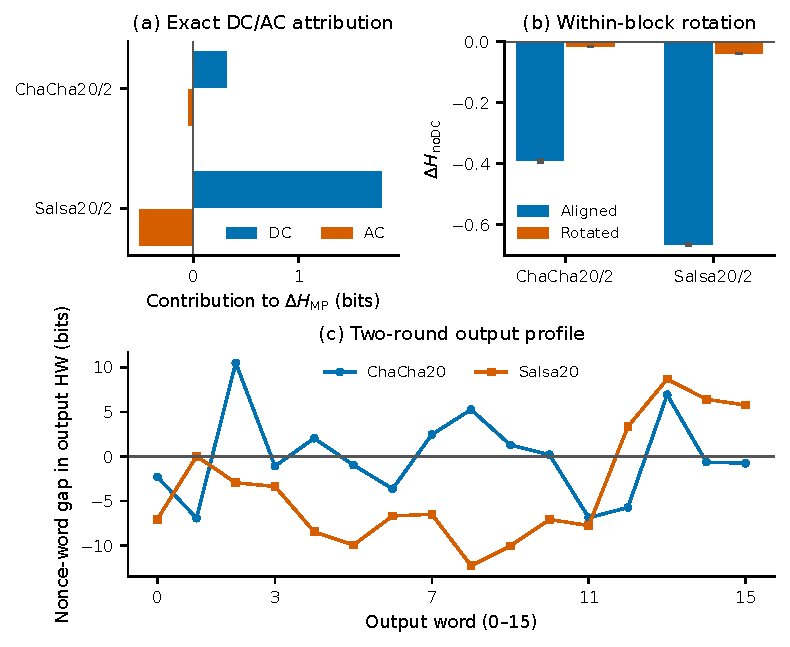
\includegraphics[width=\textwidth]{publication_unified_mask_followup}
\caption{Progressive localization of the two-round ARX response. (a) Exact DC and AC contributions to the full-spectrum entropy contrasts in the original ChaCha20 and Salsa20 cohorts. (b) Matched-nonce AC contrasts before and after 128 paired within-block cyclic rotations, which preserve each trajectory's HW values and DC share. (c) In a separate 80-key full-mask cohort, the second-minus-first nonce-word gap in 32-bit output-word HW at two rounds, pairing identical bit offsets. Error bars in (b) and bands in (c) are pointwise 95\% whole-key bootstrap intervals. The analyses use distinct cohorts as detailed in the text.\label{fig:unified}}
\end{figure}

\subsection{An Independent 64-Mask Scan Resolves Nonce-Word Responses}

The earlier four-mask scan mixed bit offsets when comparing nonce words. The independent 64-mask scan removes that ambiguity by pairing each offset across the two words. Table~\ref{tab:mask} gives the planned Salsa20/2 gap and cross-core contrast alongside the descriptive ChaCha20/2 gap. Every Salsa20 key-level average and every bit-offset average has a positive second-minus-first gap. In a descriptive round scan, the Salsa20 gap falls to $+0.00069$ bits [$-0.00018$, $0.00160$] by four rounds and remains near zero at 20.

\begin{table}[H]
\caption{Independent, position-matched 64-mask scan at two core rounds. $G_2$ is the second-minus-first nonce-word difference in observed-minus-control $H_{\rm MP}$, averaging 32 paired bit offsets per key ($Q=4$ IV pairs per mask; 80 new keys). Intervals are paired whole-key 95\% bootstrap intervals. The Salsa20 gap and the cross-core difference were planned and Holm-corrected together; the ChaCha20 row is descriptive.\label{tab:mask}}
\footnotesize\setlength{\tabcolsep}{4pt}
\begin{tabularx}{\textwidth}{lCC}
\toprule
\textbf{Contrast} & \textbf{$G_2$ [95\% CI], bits} & \textbf{Holm $p$}\\
\midrule
ChaCha20 & $-0.00036$ [$-0.00393$, $+0.00307$] & Descriptive\\
Salsa20 & $+0.79059$ [$+0.78404$, $+0.79729$] & $2.0\times10^{-5}$\\
Salsa20 $-$ ChaCha20 & $+0.79095$ [$+0.78311$, $+0.79886$] & $2.0\times10^{-5}$\\
\bottomrule
\end{tabularx}
\end{table}

The 16-position, 32-bit output-word profile reveals what the aggregate gap hides (Figure~\ref{fig:unified}c). Relative to control, Salsa20/2 second-word nonce masks yield about 14.5 fewer flipped bits per 128-bit segment than matched first-word masks. Their DC-share contrast is lower by 0.281, while normalized AC entropy is higher by 0.057. The higher full-spectrum entropy therefore reflects a weaker mean response, not more uniform output. ChaCha20/2 has almost no aggregate gap because large positive and negative output-word responses cancel. These word-level profiles are descriptive rather than planned tests.

Descriptively, the three literature-guided masks show large emitted-stream $\Delta H_{\rm MP}$ contrasts at two rounds that approach zero by four rounds. Their published internal-state biases are a different observable.

\subsection{Fresh Grain-128 Validation and Trivium Subcubes}

Fresh Grain-128 keys validate the preselected zero-clock bit-64-minus-bit-0 $\Delta H_{\rm MP}$ gap: $+0.09526$ bits [0.08921, 0.10126], with sign-flip $p\leq1.0\times10^{-5}$. Neighboring bits show similar early responses, so the effect spans an IV region rather than one exceptional position. The contrast is small after the standard 256 initialization clocks.

The Trivium subcube assay measures a different response: the fraction of one bits in a 512-bit higher-order IV derivative. For the degree-6 cube, this fraction rises from 0.1012 at 192 clocks to 0.2885 at 384 and approaches the control value of 0.5 by 768. All six degree--clock contrasts at 192 and 384 clocks survive the 12-cell max-$|t|$ correction ($p\leq2.0\times10^{-5}$), while none does at 768 or 1152. These sampled responses trace a short-initialization differential front. The conditional 24-dimensional attack uses additional key conditions beyond this pilot~\citep{knellwolf2011}.

\subsection{A5/1 Exposes a Boundary of the Diagnostic}

The preselected A5/1 flip-fraction test at 20 warm-up clocks finds no resolved contrast ($p=0.719$). At the standard 100 clocks, no cell in the corrected 44-test frame-mask search passes correction (minimum adjusted $p=0.669$). A separate fresh-key cohort does validate the selected zero-clock frame-bit-21-minus-bit-0 gradient: $-0.04350$ [$-0.05433$, $-0.03281$], $p=1.0\times10^{-5}$. Its 100-clock counterpart is small. Thus this frame test locates a shortened-initialization effect but does not track A5/1's known state-recovery weaknesses.

\subsection{Comparison with Simpler Tests on Identical Streams}

Table~\ref{tab:benchmark} compares direct and spectral statistics on the same matched-nonce streams. All six two-round contrasts have pointwise intervals excluding zero, while their four- and 20-round intervals contain zero. Mean HW and the bitwise avalanche score reveal the response deficit. Lag-four autocorrelation and position range reveal its periodic form. The positive full-spectrum contrast alongside negative AC entropy shows why spectral decomposition is useful even when simpler tests also detect the effect. Paired rotations then identify within-block alignment as the main source of that AC pattern. These unlike metrics do not support a ranking of detector sensitivity.

\begin{table}[H]
\caption{Descriptive observed-minus-control contrasts for two-round ChaCha20 and Salsa20 on the \emph{same} 80 matched-nonce keys, 16 single-bit nonce pairs, and 4096 output bits per pair. Brackets give pointwise 95\% whole-key bootstrap intervals. The bitwise score is a finite-sample strict-avalanche-style RMS deviation from flip probability $1/2$; it is not a formal SAC proof.\label{tab:benchmark}}
\footnotesize\setlength{\tabcolsep}{4pt}
\begin{tabularx}{\textwidth}{lCC}
\toprule
\textbf{Statistic} & \textbf{ChaCha20/2} & \textbf{Salsa20/2}\\
\midrule
Mean XOR HW, bits per 128 & $-21.77$ [$-22.11$, $-21.43$] & $-37.57$ [$-37.78$, $-37.37$]\\
Bitwise avalanche RMS & $+0.1844$ [$+0.1822$, $+0.1866$] & $+0.2952$ [$+0.2939$, $+0.2965$]\\
Lag-four HW autocorrelation & $+0.6877$ [$+0.6776$, $+0.6979$] & $+0.8887$ [$+0.8796$, $+0.8975$]\\
Four-position HW range, bits & $+17.87$ [$+17.53$, $+18.21$] & $+30.41$ [$+30.03$, $+30.78$]\\
Full-spectrum entropy, bits & $+0.2648$ [$+0.2590$, $+0.2707$] & $+1.2529$ [$+1.2408$, $+1.2646$]\\
Normalized AC entropy & $-0.3912$ [$-0.3963$, $-0.3860$] & $-0.6657$ [$-0.6677$, $-0.6637$]\\
\bottomrule
\end{tabularx}
\end{table}



\section{Discussion}

Spectral entropy summarizes the frequency allocation of a paired-IV output-difference trajectory. The graph-matched control flags departures; DC share and AC entropy distinguish their causes. Grain-128 and Trivium show mostly transient DC-linked deficits, while two-round ChaCha20 and Salsa20 show persistent block-position structure with an AC contribution opposite to the full-spectrum sign. Direct HW and avalanche tests detect the large two-round deficits, and the four-position HW range and autocorrelation expose their periodicity. The spectral statistic therefore offers a compact decomposition and a route to localization, not demonstrated superiority in detection.

The paired rotations sharpen the output interpretation: they preserve HW values, length, and DC share while removing about 96\% and 94\% of the original two-round ChaCha20 and Salsa20 AC contrasts. The new 64-mask scan removes the earlier within-word bit-offset confound. Salsa20/2 has a net second-word deficit in HW and DC share; ChaCha20/2 has a much smaller aggregate gap, but opposing 32-bit output-word responses cancel in the 128-bit summary. Grain's replicated IV-region gradient and Trivium's short-initialization subcube front localize other effects; the latter probes higher-order differential response, not spectral entropy.

A5/1 marks a useful boundary. Its independently validated zero-clock gradient shows that the frame test can see delayed diffusion when initialization is removed. Yet a corrected search over standard 100-clock frame responses found no signal, despite published A5/1 attacks~\citep{biryukov2000}. Those attacks concern state recovery, which this test does not measure. A quiet IV-response screen is therefore compatible with a cryptanalytically weak cipher.

The original fresh-key, Salsa20-transfer, phase-rotation, full-mask, and A5/1 standard-search tests were fixed before their cohorts. The earlier four-mask nonce-word comparison and the new output-word profiles are descriptive. The selected Grain and A5/1 zero-clock contrasts were tested on separate fresh keys. Cipher grids do not represent equal internal work, SHAKE256 is a computational control, and the Trivium pilot omits published weak-key conditions. These finite cohorts leave broader random-function behavior unresolved. These diagnostics do not rank security or bound attack advantage.

\Needspace{8\baselineskip}
\section{Conclusions}

Phase-aware spectral entropy can screen how IV changes propagate through stream-cipher output. Standard settings showed small contrasts, reduced Grain-128 and Trivium had transient effects, and two-round ChaCha20 and Salsa20 had persistent block-position structure. Matched-nonce rotations attributed most of the reduced cores' AC anomaly to within-block alignment. Crucially, the independently planned 64-mask scan confirmed a $+0.79059$-bit second-minus-first nonce-word gap in Salsa20/2 after matching bit offsets (Holm-adjusted $p=2.0\times10^{-5}$). ChaCha20/2 had a near-zero aggregate gap, yet its 16-word output profile revealed large compensating responses. The contrast distinguishes a net Salsa20 deficit from a ChaCha20 redistribution hidden by aggregation.

The new Grain-128 cohort replicated an early IV-region gradient; smaller Trivium cubes exposed a short-initialization differential front that was no longer detected at 768 clocks. A5/1 independently replicated a zero-clock frame-position gradient ($-0.04350$ in bit-21-minus-bit-0 flip fraction), but no 100-clock mask passed a corrected 44-cell search. This known vulnerable cipher illustrates the scope of the test: it can localize delayed IV diffusion while missing weaknesses based on state recovery. The large ARX effects vanish from our aggregate contrasts by four rounds, and direct same-stream statistics also detect their early deficits. None of these results estimates keystream Shannon entropy, demonstrates a full-round weakness, or quantifies attack advantage.

\authorcontributions{Conceptualization, methodology, software, validation, formal analysis, investigation, data curation, visualization, writing---original draft, and writing---review and editing, P.A. The author has read and agreed to the published version of the manuscript.}
\funding{This research received no external funding.}
\institutionalreview{Not applicable.}
\informedconsent{Not applicable.}
\dataavailability{The versioned reviewer archive contains fixed protocols, raw trajectories, higher-order derivatives and paired frame XORs, per-key and summary results, planned and descriptive mask analyses, vector checks, code, and SHA-256 hashes for all cohorts. No public DOI has yet been assigned; it will be added after deposition.}
\conflictsofinterest{The author declares no conflicts of interest.}
\begin{adjustwidth}{-\extralength}{0cm}
\reftitle{References}
\bibliography{biblio}
\end{adjustwidth}
\end{document}
